\section{Use cases diagramm}
\subsection{Description}
\begin{flushleft}
Pour commencer, nous regardons les différentes fonctionnalités à implémenter via ce diagramme. Tout d'abord, l'application permet à un client de visualiser l'historique de ses factures ainsi que les acomptes mensuels et leur statut de paiement.
\end{flushleft}

\begin{flushleft}
Ensuite, un client peut accéder au montant de l'acompte mensuel proposé par l'application. Celui-ci est calculé automatiquement, basé sur les rapport énergétiques annuels du client, du coût de l'énergie actuel et des installations du client. L'utilisateur peut donc, soit accepter la proposition ou la refuser en proposant une alternative.\footnote{Comprise en +-20% en fonction de la modification}
\end{flushleft}

\begin{flushleft}
De plus, lorsque celles-ci sont erronées, le client peut modifier ses informations bancaires. Dans le cas où le client a choisi une domiciliation, il est possible pour celui-ci de modifier les informations reliés à son compte bancaire.
D'autre part, le client peut modifier ce mode paiement et basculer du mode automatique à mannuel (ou inversément).
\end{flushleft}

\begin{flushleft}
Enfin, le client peut procéder au paiement de sa facture. Celui-ci pourra donc générer un QR code lui permettant d'effectuer un virement bancaire plus simple.
\end{flushleft}

\begin{figure}[h]
\subsection{Schéma}
\centering
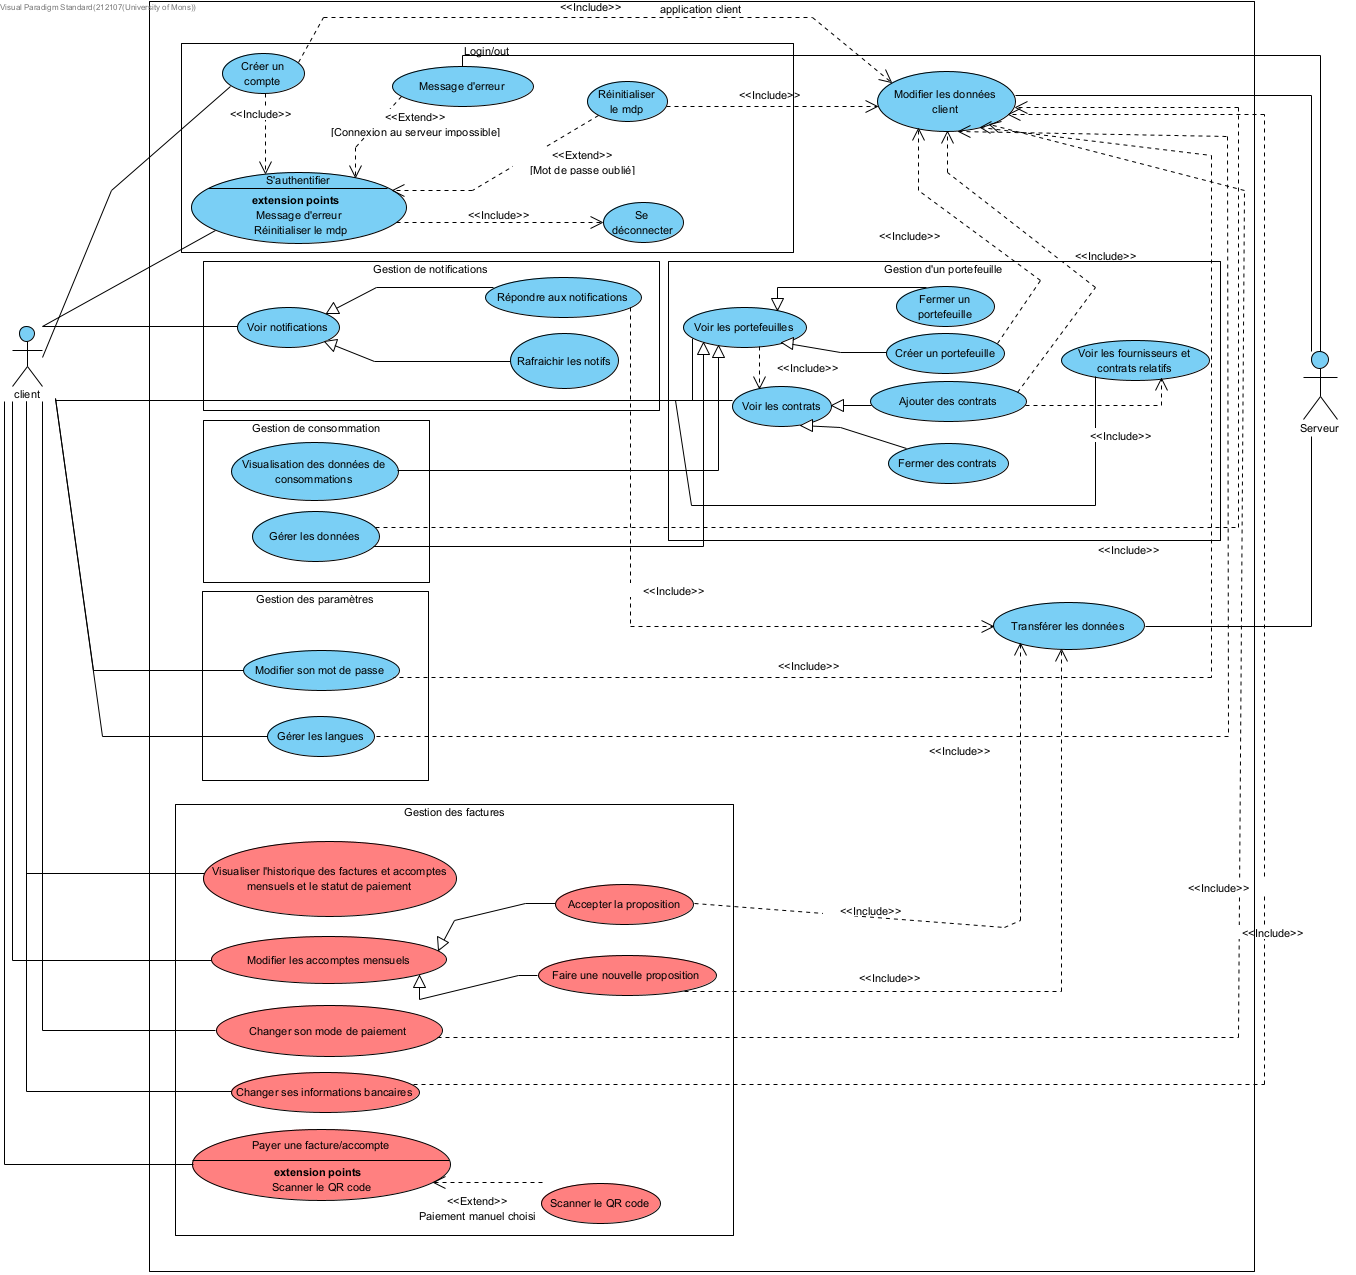
\includegraphics[width = 1\textwidth]{extension-maxime/usescases/img/usecases-extension.png}
\end{figure}



